\documentclass[11pt,a4paper]{article}
\usepackage[utf8]{inputenc}\usepackage[T1]{fontenc}
\usepackage{amsmath,amssymb,amsthm}
\usepackage[margin=1in]{geometry}
\usepackage{graphicx}\usepackage{mathrsfs}
\usepackage[hidelinks]{hyperref}
\newtheorem{theorem}{Theorem}
\newtheorem{corollary}{Corollary}
\newtheorem{lemma}{Lemma}
\newtheorem{definition}{Definition}

\title{\Large \textbf{The Irreducible Three-Body Congruence Correlation\\
and the Annihilation Lattice on the $6N$ Skeleton}}
\author{Ruqing Chen\\
\small GUT Geoservice Inc., Montreal, Quebec, Canada\\
\small \texttt{ruqing@hotmail.com}}
\date{\today}

\begin{document}
\maketitle

\begin{abstract}
Part~XX recast the two-centre correlation of prime constellations as a circular
convolution of castellated indicators on the phase-space torus $\mathbb{T}^1$.
Here we extend the phase-space integration to three twin centres and ask whether
the three-body correlation factorises into pairwise interactions. It does not. We
define the irreducible three-body factor $U(j_1,j_2)=R_3/(R_2(j_1)R_2(j_2)
R_2(j_2-j_1))$ and find $U\neq1$ at \emph{every} lag pair: a genuine irreducible
three-body congruence term is generic, not exceptional. We then state the correct
criterion for total annihilation ($R=0$): the union of the constellations'
dead-residue sets must \emph{tile} $\mathbb{Z}/q$ for some prime $q$. This
corrects a natural but false dimension-count heuristic ($m_A+m_B\ge q$): tiling
requires the hole-sets to be \emph{complementary}, not merely numerous. A triplet
contains a twin, so their dead-sets always overlap and a Twin--Triplet pair never
annihilates ($I_q\ge1/q>0$); the lowest order at which twin-based annihilation
occurs is therefore \emph{three}-body---three consecutive twin centres tile
$\mathbb{Z}/5$, recovering the mod-$5$ inadmissibility of a six-member skeleton
window. We map the resulting annihilation lattice and the finite irreducible term.
Closed-form throughout; the integral equals the discrete singular-series ratio at
integer lags; no infinitude is claimed.
\end{abstract}

\section{Introduction}
Part~XX established that the spatial correlation of two twin centres is a circular
convolution of castellated indicators on $\mathbb{T}^1$, quantised into three
interference states~\cite{ChenXX}. A two-body correlation, however, cannot by
itself reveal whether the lattice of twin centres behaves as a gas of independent
pairs or carries genuine higher-order structure. The natural next question is
whether the three-body correlation $R_3(j_1,j_2)$ of twins at $N$, $N+j_1$,
$N+j_2$ factorises into the product of the three pairwise correlations of Part~XX.

We show it does not, anywhere. The deviation defines an \emph{irreducible
three-body congruence term} that is generic across the lattice, and whose extreme
limit---total annihilation, $R_3=0$---obeys a precise tiling criterion that we
state and that corrects a tempting dimension-count heuristic. As in Volume~I, we
separate axes carefully: the annihilation studied here is a \emph{horizontal}
(inter-centre) phenomenon, distinct from the single-centre ``killer prime'' that
drives the \emph{vertical} $\omega$-collapse of Volume~I~\cite{ChenXVII,Review}.

\section{The three-body joint measure}
For a prime $q>3$ a twin centre $N$ is forbidden modulo $q$ on the two dead
residues $\mathrm{dead}(q)=\{6^{-1},-6^{-1}\}$. A twin at $N+j$ has the shifted set
$\mathrm{dead}(q)-j\pmod q$. For twins at $N,N+j_1,N+j_2$ (taking $j_0=0$) the
joint survival measure at $q$ is the transmitting fraction of the union,
\begin{equation}
  I_q(j_1,j_2)=\frac{q-\nu_q}{q},\qquad
  \nu_q=\Big|\,\mathrm{dead}(q)\,\cup\,(\mathrm{dead}(q)-j_1)\,\cup\,(\mathrm{dead}(q)-j_2)\,\Big|,
\end{equation}
and the normalised three-body correlation, with $\mathfrak{S}$ the singular series, is
\begin{equation}
  R_3(j_1,j_2)=\frac{\mathfrak{S}(\text{all three})}{\mathfrak{S}_{\rm twin}^3}
  =\prod_{q>3}\frac{1-\nu_q/q}{(1-2/q)^3}.
\end{equation}
The pairwise correlation of Part~XX is $R_2(j)=\prod_q (1-\nu_q^{(2)}/q)/(1-2/q)^2$
with $\nu_q^{(2)}=|\mathrm{dead}(q)\cup(\mathrm{dead}(q)-j)|$.

\begin{definition}[Irreducible three-body factor]
\begin{equation}
  U(j_1,j_2)\;=\;\frac{R_3(j_1,j_2)}{R_2(j_1)\,R_2(j_2)\,R_2(j_2-j_1)} .
\end{equation}
$U\equiv1$ would mean the three-body correlation is fully explained by its three
pairwise interactions. Any deviation is an irreducible three-body term.
\end{definition}

By inclusion--exclusion, $\nu_q=\sum|A_i|-\sum|A_i\cap A_j|+|A_1\cap A_2\cap A_3|$;
the three pairwise factors absorb the singletons and the pairwise intersections,
so $U$ is driven by the triple intersection $|A_1\cap A_2\cap A_3|$---a residue
killed by all three centres at once---together with the saturation that occurs
when the union fills $\mathbb{Z}/q$.

\section{The annihilation criterion: tiling, not counting}
\begin{theorem}[Annihilation is tiling]\label{thm:tile}
The joint density of constellations $A_1,\dots,A_k$ at centres $N+j_1,\dots,N+j_k$
vanishes, $R=0$, if and only if there exists a prime $q>3$ at which the shifted
dead-sets cover every residue,
\[
  \bigcup_{i=1}^{k}\big(\mathrm{dead}_{A_i}(q)-j_i\big)=\mathbb{Z}/q\mathbb{Z}.
\]
\end{theorem}
\begin{proof}
$R=0$ iff some local factor $1-\nu_q/q=0$, i.e.\ $\nu_q=q$, i.e.\ the union of the
shifted dead-sets is all of $\mathbb{Z}/q$. A single vanishing prime annihilates
the whole product.
\end{proof}

This makes precise---and corrects---the intuition that ``dimension sum
$\ge q$ forces collapse.'' Covering $\mathbb{Z}/q$ requires the dead-sets to
\emph{tile}: to be numerous \emph{and} complementary. Mere counting is not enough.

\begin{corollary}[No Twin--Triplet annihilation]\label{cor:tt}
A triplet $(6N-1,6N+1,6N+5)$ contains the twin $(6N-1,6N+1)$, so at $q=5$
$\mathrm{dead}_{\rm trip}(5)=\{0,1,4\}\supseteq\{1,4\}=\mathrm{dead}_{\rm twin}(5)$.
For every shift $j$ the two sets overlap, $\mathrm{dead}_{\rm twin}\cap
(\mathrm{dead}_{\rm trip}-j)\neq\varnothing$, so they can never tile $\mathbb{Z}/5$;
direct evaluation gives $I_5(j)\in\{1/5,2/5\}$, never $0$. A Twin--Triplet pair
does not annihilate at any lag; indeed no two-body pair built on a shared twin
does. The twin's two-hole budget is simply too small to complete a tiling against
a partner that already contains it.
\end{corollary}

The lowest order at which twin-based annihilation can occur is thus $k=3$: three
twins contribute $2k=6\ge5$ holes, enough to tile the smallest prime $q=5$.

\section{The irreducible term and the annihilation lattice}
Evaluating $U(j_1,j_2)$ over the lattice $1\le j_1,j_2\le30$ (singular-series
cutoff $q\le59$) gives the central empirical facts of this paper, shown in
Fig.~\ref{fig:three}.

\begin{figure}[h]\centering
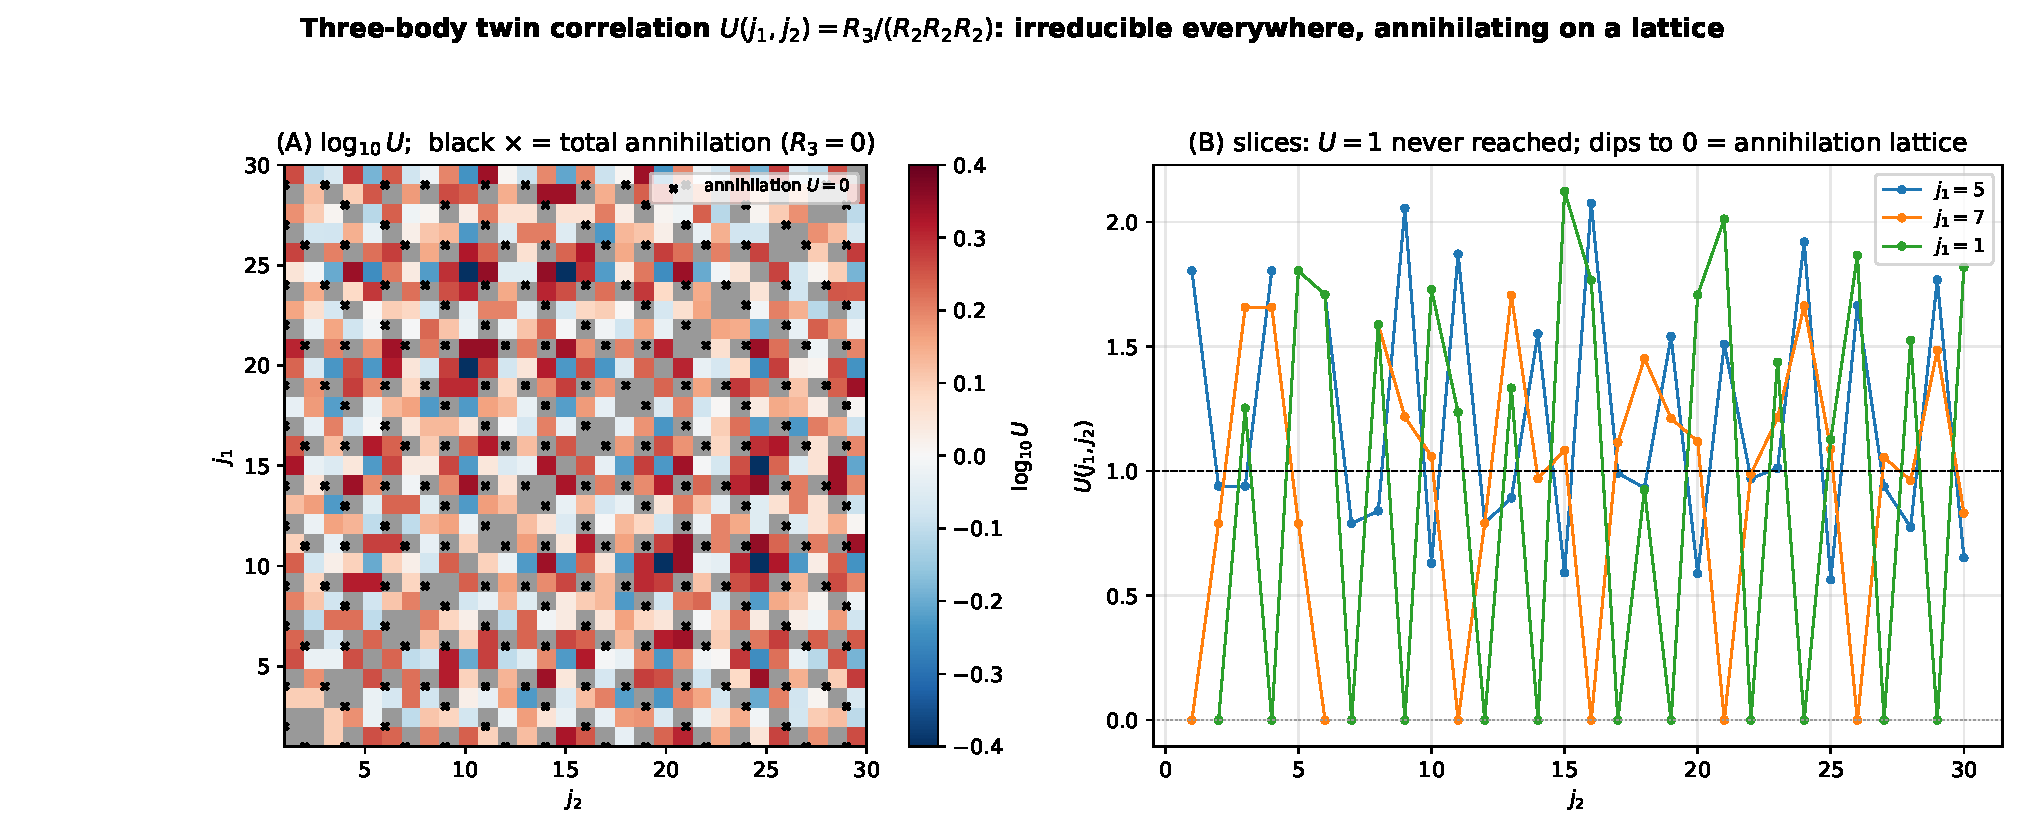
\includegraphics[width=0.97\textwidth]{fig_three_body.pdf}
\caption{(A) $\log_{10}U(j_1,j_2)$ for three twin centres; black crosses mark the
annihilation lattice $U=0$ ($R_3=0$). (B) Slices $j_1\in\{1,5,7\}$: $U=1$
(independence of the three-body term) is reached nowhere, and the curve dips to
$0$ on the annihilation lattice.}
\label{fig:three}
\end{figure}

\noindent\textbf{Three-body terms are generic.} Across all $870$ ordered lag pairs
in the window, $U=1$ occurs \emph{nowhere}: the three-body correlation never
reduces to its pairwise parts. The finite irreducible term ranges from $U\approx
0.37$ to $U\approx2.24$; its sharpest finite values arise from a triple
coincidence, a prime at which all three centres share a dead residue (e.g.\
$j_1=5,j_2=10$, where $0,5,10$ are all $\equiv0\pmod5$ and the three twin holes
align, $|A_1\cap A_2\cap A_3|=2$ at $q=5$).

\noindent\textbf{The annihilation lattice.} Of the scanned pairs, $216$ give
$U=0$: a periodic lattice of forbidden configurations. The defining instance is
$(j_1,j_2)=(1,2)$---three consecutive twin centres. At $q=5$,
\[
  \{1,4\}\cup(\{1,4\}-1)\cup(\{1,4\}-2)=\{1,4\}\cup\{0,3\}\cup\{2,4\}=\mathbb{Z}/5,
\]
so the six skeleton members $6N-1,6N+1,6N+5,6N+7,6N+11,6N+13$ always contain a
multiple of $5$: three consecutive twin centres are impossible beyond $6N=5$.
Theorem~\ref{thm:tile} thus reproduces, from pure phase-space tiling, the
mod-$5$ inadmissibility that classical $k$-tuple theory assigns to this
six-member window. The annihilation lattice is the admissibility constraint seen
as a congruence diffraction zero.

\section{Twin immunity, restated}
\begin{lemma}[Two-body twin immunity]
No two-body correlation built on a twin annihilates: for any partner $X$,
$R_2=0$ would require $\mathrm{dead}_{\rm twin}(q)$ and $\mathrm{dead}_X(q)-j$ to
tile $\mathbb{Z}/q$, impossible for $q\ge5$ whenever the partner shares the twin's
members (Corollary~\ref{cor:tt}). In particular Twin--Twin has
$I_q\ge(q-4)/q\ge1/5>0$.
\end{lemma}

We stress what this does \emph{not} say. Two-body immunity is not unique to the
twin, and it is not the source of the Volume~I ``killer prime'' collapse. That
collapse is a \emph{single-centre} effect---a cross-centre tuple's own member
$6N+5$ is divisible by $5$ whenever $5\mid N$, i.e.\ $0\in\mathrm{dead}(5)$---and
lives on the vertical $\omega$-axis~\cite{ChenXVII}. The horizontal annihilation
of this paper is a distinct, higher-order phenomenon: it needs three bodies, and
it encodes admissibility rather than divisibility of a single member.

\section{Conclusion}
Extending the phase-space convolution to three centres shows that the lattice of
twin centres is not a gas of independent pairs: an irreducible three-body
congruence term is present at every lag, and its zeros form a periodic
annihilation lattice governed by a tiling criterion (Theorem~\ref{thm:tile}). The
criterion corrects the naive dimension count---tiling demands complementarity, not
abundance---and explains why a Twin--Triplet pair, despite $m_A+m_B=5$, never
annihilates, while three consecutive twins do, recovering mod-$5$ admissibility
from geometry alone. The natural next step is the general $k$-body tiling spectrum
and its relation to the Hardy--Littlewood admissibility of long windows on the
$6N$ skeleton. As throughout the programme, the construction is closed-form, equal
to the discrete singular-series ratio at integer lags, and makes no claim about
the infinitude of any constellation.

\paragraph{Data and code availability.}
The three-body computation (the irreducible factor $U$, the annihilation count,
and the figure) and a verifier of the tiling criterion are openly
available~\cite{repo}.

\begin{thebibliography}{9}
\bibitem{HL} G.~H.~Hardy, J.~E.~Littlewood, \emph{Some problems of `Partitio
Numerorum'; III}, Acta Math.\ \textbf{44} (1923), 1--70.
\bibitem{ChenI} R.~Chen, Part~I, Zenodo, doi:10.5281/zenodo.20470367 (2026).
\bibitem{ChenXII} R.~Chen, Part~XII, Zenodo, doi:10.5281/zenodo.20528446 (2026).
\bibitem{ChenXVII} R.~Chen, \emph{Arithmetic geodynamics on the $6N$ skeleton}
(Part~XVII), Zenodo, doi:10.5281/zenodo.20541575 (2026).
\bibitem{ChenXIX} R.~Chen, \emph{The tuple-size law at $m=5$} (Part~XIX), Zenodo,
doi:10.5281/zenodo.20551393 (2026).
\bibitem{ChenXX} R.~Chen, \emph{The circular convolution of prime constellations
in congruence phase space} (Part~XX), Zenodo, doi:10.5281/zenodo.20583994 (2026).
\bibitem{Review} R.~Chen, \emph{Arithmetic geodynamics on the $6N$ skeleton: a
review of Parts I--XIX}, \url{https://github.com/Ruqing1963/6N-review} (2026).
\bibitem{repo} R.~Chen, \emph{The irreducible three-body congruence correlation
and the annihilation lattice} (Part~XXI),
\url{https://github.com/Ruqing1963/6N-three-body} (2026).
\end{thebibliography}

\end{document}
